	\setlength{\tabcolsep}{3pt}
	\null\vfill\null
	\begin{center}
	\parbox{\textwidth-2\tabcolsep}{
		\begin{center}
			$\left.\begin{array}{cl} \text{10.\,Ky\={u}} & \raisebox{-7.2pt}{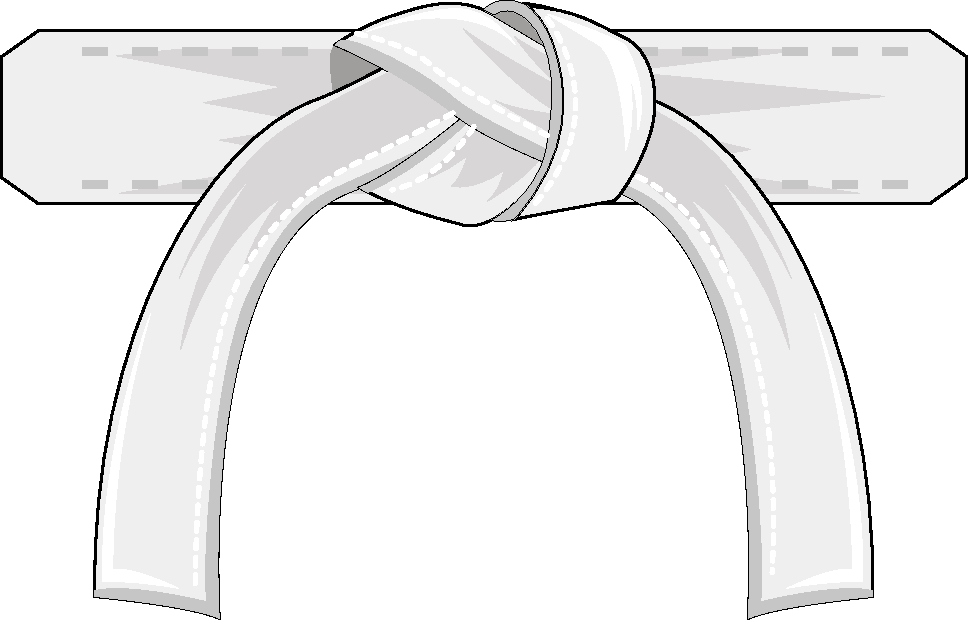
\includegraphics[height=24pt]{Gfx/gurte/whitebelt}}\\ \text{9.\,Ky\={u}} & \raisebox{-7.2pt}{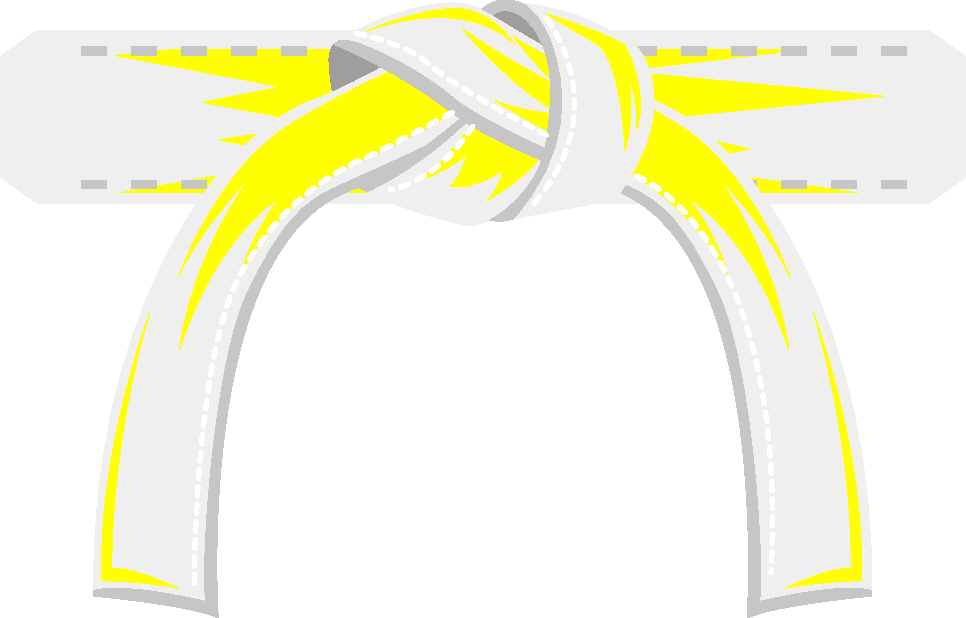
\includegraphics[height=24pt]{Gfx/gurte/whiteyellowbelt}}\\ \text{8.\,Ky\={u}} & \raisebox{-7.2pt}{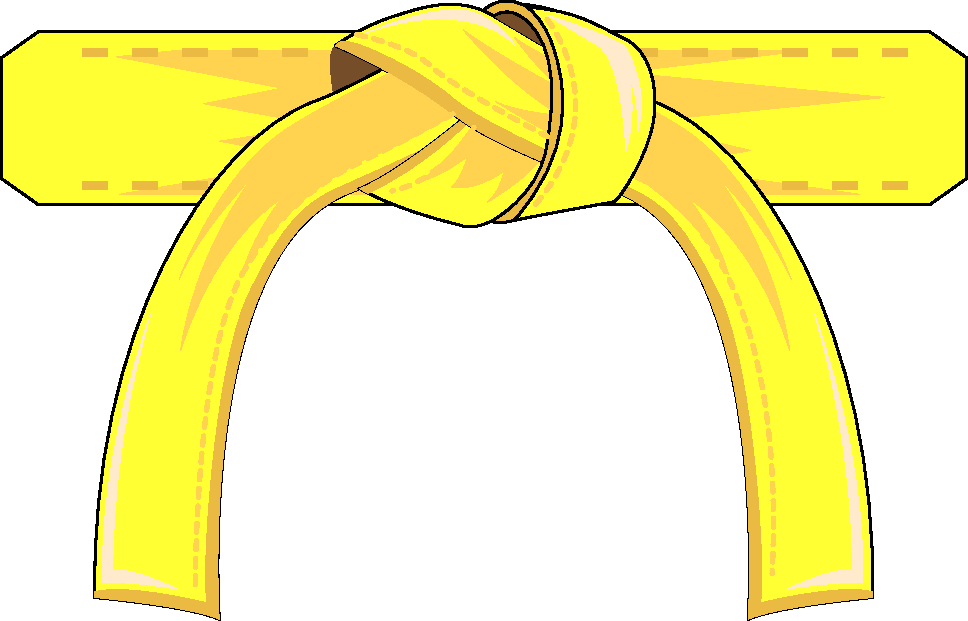
\includegraphics[height=24pt]{Gfx/gurte/yellowbelt}}\\ \text{8.\,Ky\={u}}& \raisebox{-7.2pt}{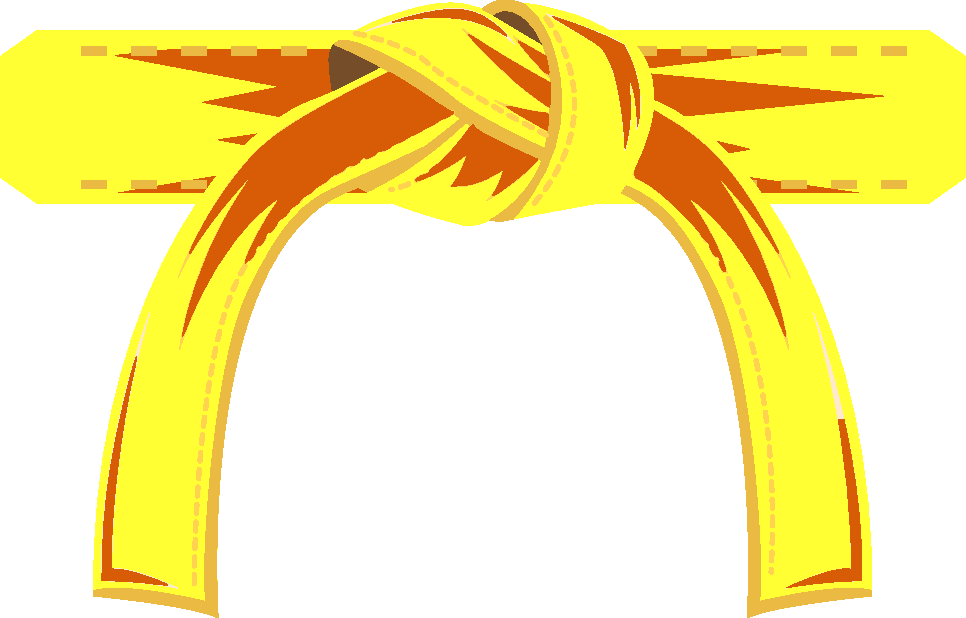
\includegraphics[height=24pt]{Gfx/gurte/yelloworangebelt}}\end{array} \right\}\text{Unterstufe}$\quad$\left.\begin{array}{cl} \text{7.\,Ky\={u}} & \raisebox{-7.2pt}{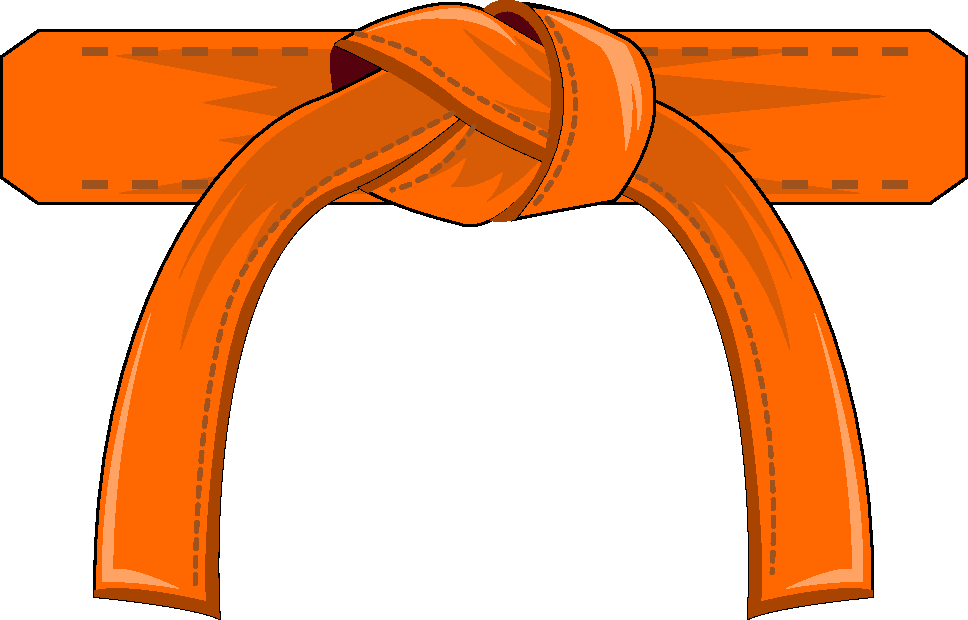
\includegraphics[height=24pt]{Gfx/gurte/orangebelt}} \\ \text{7.\,Ky\={u}} & \raisebox{-7.2pt}{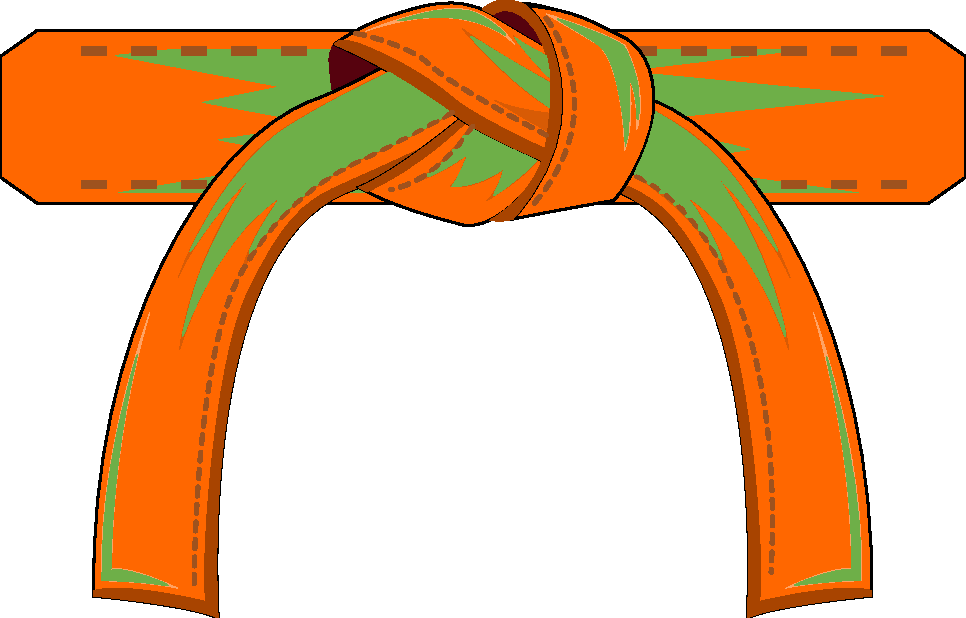
\includegraphics[height=24pt]{Gfx/gurte/orangegreenbelt}}\\ \text{6.\,Ky\={u}} & \raisebox{-7.2pt}{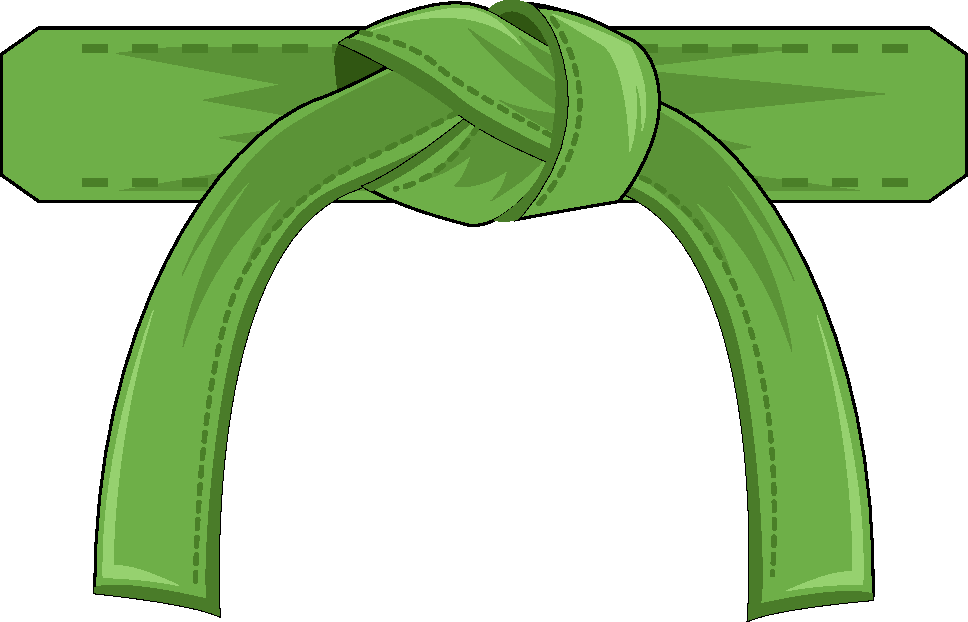
\includegraphics[height=24pt]{Gfx/gurte/greenbelt}}\\ \text{5.\,Ky\={u}} & \raisebox{-7.2pt}{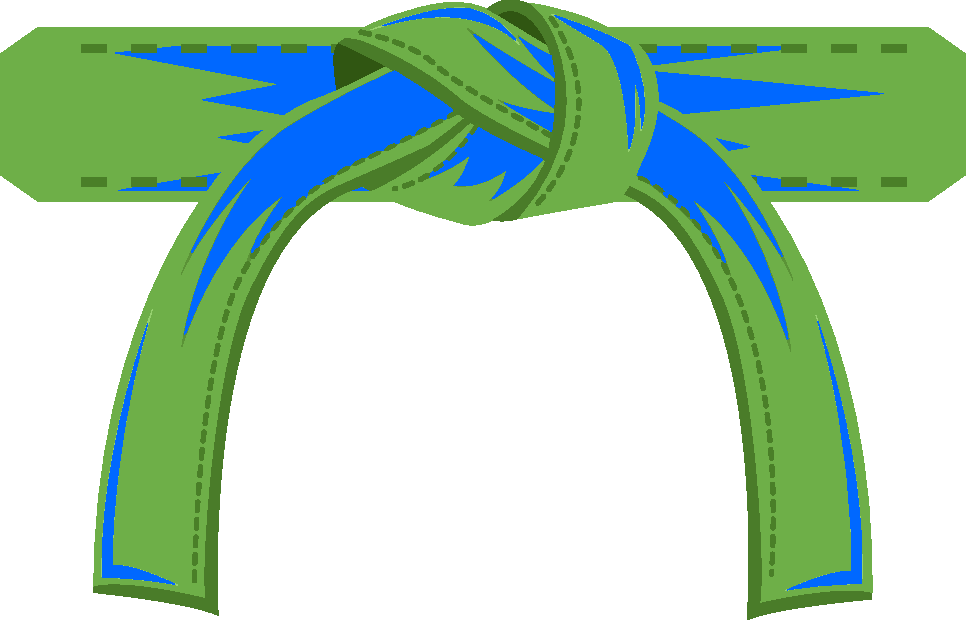
\includegraphics[height=24pt]{Gfx/gurte/greenbluebelt}}\end{array} \right\}\text{Mittelstufe}$\quad$\left.\begin{array}{cl} \text{5.\,Kyu} & \raisebox{-7.2pt}{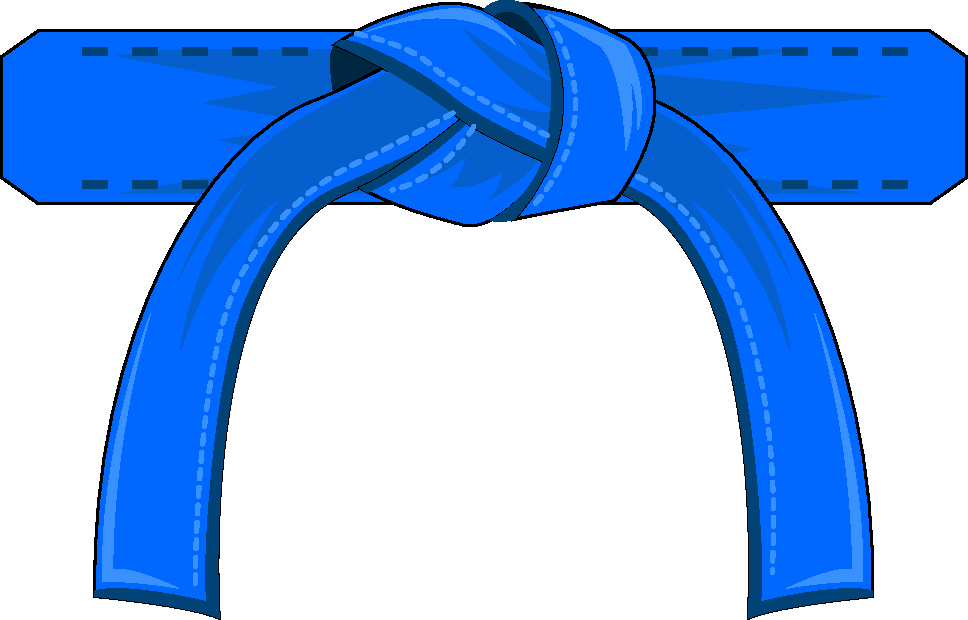
\includegraphics[height=24pt]{Gfx/gurte/bluebelt}}\\ \text{4.\,Ky\={u}} & \raisebox{-7.2pt}{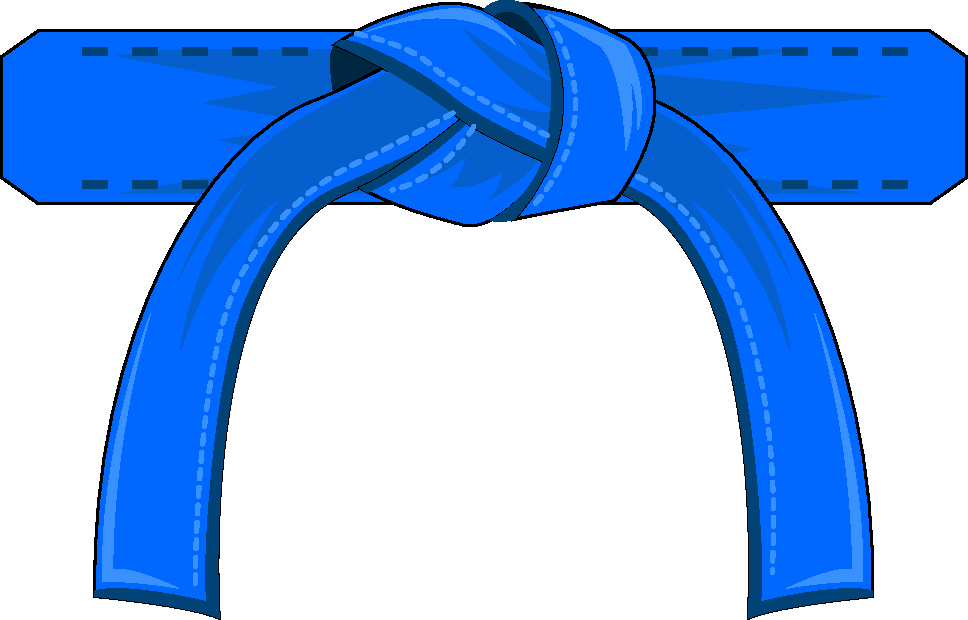
\includegraphics[height=24pt]{Gfx/gurte/bluebelt}} \end{array} \right\}\text{Oberstufe}$
		\end{center}
		Die Ky\={u}grade werden in unserem Dojo meist von euren Trainern geprüft. Das Prüfungsprogramm, also die zugrunde liegenden Techniken, Partnerformen und Katas, sind auf den entsprechenden Trainingskarten aufgelistet. \textit{\underline{Anmerkun}}g: die Prüfung zum 4.\,Ky\={u} bedeutet häufig den Übergang in den Erwachsenenbereich.\\

		Die Prüfungen finden meist 2\textit{x}\, pro Jahr statt, damit ein gutes Mittelmaß zwischen Fortschritt in der Gürtelfarbe und grundlegendem Training der notwendigen Techniken gewährleistet ist\\}

%		\textit{Besonderheiten unseres Dojo:} Der Prüfungsinhalt zum 1.\,Kyu umfasst, zusätzlich zum eigentlichen Programm, auch die Inhalte der ebenfalls an diesem Tag stattfindenden Prüfungen - wenn zum Beispiel zur Prüfung zum 1.\,Kyu zwei Karateka angemeldet sind, sowie jeweils ein Karateka zum 9.,\,5.\,und 7.\,Kyu, so gehen die beiden zuerst genannten die jeweiligen Prüfungsprogramme der anderen ebenfalls mit - mit Ausnahme von Partnerformen und Kata-Bunkai. Findet an diesem Tag keine andere Prüfung statt, werden weitere Prüfinhalte im Vorfeld abgesprochen.
	\end{center}\null\vfill\null
	\setlength{\tabcolsep}{6pt}